\setlength{\parskip}{.2em}
\graphicspath{ {./chapter-3/figures/} }
\captionsetup[figure]{labelfont=bf}
\captionsetup{margin=1.5em}
\captionsetup[table]{labelfont=bf}


\chapter{Landscape exploration with simple systems}
\label{chapter_3}

%% The following annotation is customary for chapter which have already been
%% published as a paper.
\blfootnote{Parts of this chapter have been published in Applied Optics \textbf{55}, 10449 (2016) \cite{HouSimple16}.}

%% It is only necessary to list the authors if multiple people contributed
%% significantly to the chapter.
%\authors{Albert {\titleshape Einstein}}

% %% The '0pt' option ensures that no extra vertical space follows this epigraph,
% %% since there is another epigraph after it.
% \epigraph[0pt]{
%   A journey of a thousand miles begins with a single step
% }{Laozi}

% \epigraph{
%     Sample quotes
% }{author}

% \begin{abstract}
% Previous researches have shown that different solutions of the optical system can be found using saddle point based method for some simplified cases\cite{PascalTriplet2009}. It is important, however, to study whether the saddle point based method still perform well in practical lens design problems. To study this, we chose to start with a relative simple example.
% \end{abstract}

% %% Start the actual chapter on a new page.
% \newpage

\noindent 
In a lens design landscape, from a saddle point system with Morse index $1$, optimization will lead to two solutions of local minima.  When performing a saddle point construction (SPC) scan \footnote{The definition of "performing an SPC scan" is given in Chapter \ref{spc-general}.}, it can find several saddle point configurations, which subsequently lead to multiple local minima. 

Therefore, it is an intriguing question whether or not the local minima in the design landscape are all connected by the saddle points of Morse index $1$. If this is the case, then by constructing sufficiently many saddle points, in principle all local minima of the design landscape can be obtained. 

This chapter is mainly based on a research paper\cite{HouSimple16} published in 2016. It is shown that in the design landscape of a wide-angle pinhole lens and in closely related optimization landscapes, all good local minima found by other methods can be obtained easily with a succession of one-dimensional searches (SPC scans) starting from simpler systems. By replacing high-dimensional searches with a succession of one-dimensional searches, the design efficiency can be increased significantly. By combining this method with conventional design methods, the wide-angle pinhole lens can be designed starting from a single lens.

% Reason for choosing the wide-angle pinhole lens. 1) Application wise, it is application wise popular. 2) It is sufficiently different from the previous studied ideal examples.
In a research paper in 2004 \cite{BociortThinLens2004}, Bociort et al. show that when a thin lens model is used, and only the spherical aberration is considered, the minima and saddle points in the lens design landscape form a network. The saddle points in this network can be theoretically predicted, hence from the saddle points, minima are obtained. A research conducted by Van Grol et al.\cite{PascalTriplet2009} claims that there is a fundamental network for a lens design problem with a certain number of lenses. In their paper, examples of the fundamental network of doublet and triplet systems have been given. The authors predict that in practical design cases, the type of system shapes \footnote{In a lens system, each lens element has its lens form: biconcave, biconvex, meniscus, etc. The type of the system shape of a lens system is determined by the combination of the individual lens forms. For example, a biconcave-biconvex doublet is one type of system shape, and a biconcave-meniscus is a different type of system shape. } of the solutions will not exceed the types of system shapes from the fundamental network. In a later research paper from 2010\cite{BociortTripletExplained2010}\cite{BociortToyModel2010}, Bociort shows that a toy model based on third-order spherical aberration can be used to mathematically explain the fundamental network of the triplet. 

For the assumption that the dominant aberration is spherical aberration, and that the lenses are not too thick, it is possible to predict the existing solutions within the network. However, in practical cases, aberrations other than spherical aberration will also determine the topology of the merit function landscape. In this case, it is mathematically too complex to build an analytical model to predict the behaviour of the merit function landscape.

Despite the complexity to use an analytic model to predict the merit function landscape, it has been shown earlier \cite{BociortSPCSexplained}\cite{MVTurnhoutSPC15} that in the lens design space a special structure is present that makes the lens design problem different from a general global optimization problem: certain saddle points existing in the landscape are reducible to minima of simpler systems with one lens element less. Using this structure, the Saddle Point Construction (SPC) \cite{MVTurnhoutSPC15} method is developed to obtain new design solutions. In the conventional approach, trial and error is needed to look for different solutions (if there is more than one) by adding one extra lens element to the existing system. With the SPC, there is a systematic procedure to search for available solutions by adding new element to the system. When starting from a minimum with $N$ variables, with SPC it is possible to systematically find minima in an $(N+2)$ dimensional variable space by using one-dimensional searches, rather than $(N+2)$ dimensional searches. Important questions are, however, how many minima existing in the landscape can be obtained in $(N+2)$ dimensional search spaces, by replacing high-dimensional searches with one-dimensional searches? What percentage of them can be found? Is it possible to at least obtain the good solutions? In this chapter, the performance of saddle point construction is evaluated for more general problems, especially those of practical interests. 


%%%%%%%%%%%%%%%%%%%%%%%%%%%%%%%%% Section 1 %%%%%%%%%%%%%%%%%%%%%%%%%%%%%%%%%%%%%%%
\section{Wide-angle pinhole lens}

A wide angle pinhole lens, designed by Irina Livshits from ITMO, has been chosen to study the design landscape using saddle point construction. This kind of lens becomes very popular in recent years for surveillance applications. Instead of a lensless optical element, the pinhole lens here refers to a lens having an aperture stop with a small diameter placed in front of the system. All lenses are in contact, one lens is cemented, and three different glass materials are used [see Figure \ref{fig:widepinLens}(a)]. The specifications are given in Table \ref{table: sysspec}. In Figure \ref{fig:widepinLens}(b) a 2D image simulation made with CODE V shows that, despite its simplicity, the system has an imaging quality that is adequate for its intended purpose. The system can also be adapted for spectral imaging applications \cite{Strauch2015}. For optimization we used the default CODE V merit function that is based on transverse ray aberrations. The value of the merit function (called in CODE V error function) for this system is 5.68 $\mu m^2$. It is a composite value, scaled so that it is the mean square of the weighted image radius. The value has considered a setting with three wavelength as shown in Table \ref{table: sysspec}. In the following text in this chapter, values of the merit function are presented without adding the unit. 

\begin{figure}[h!]
    \centering
    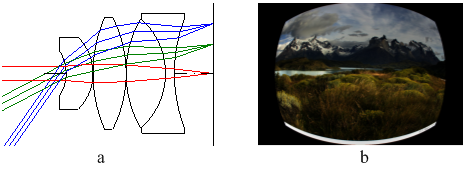
\includegraphics[scale=0.95]{chapter-3/figures/WidePinLens.png}
    \caption{Wide-angle pinhole lens. (a) Lens drawing. (b) 2D image simulation of its imaging quality.}
    \label{fig:widepinLens}
\end{figure}

\setlength{\arrayrulewidth}{.5mm}
\setlength{\tabcolsep}{18pt}
\renewcommand{\arraystretch}{1.2}
\begin{table}[h!]
    \centering
    \captionsetup{justification=centering}
    \caption{System specification}
    \label{table: sysspec}
    \vspace{-1em}
    \begin{tabular}{ p{20em} c }
    \hline 
    Entrance pupil diameter (EPD, mm) & 0.8\\
    Full field of view (FOV, °) & 110\\
    Effective focal length (EFL, mm) & 3.5\\
    Wavelength (nm) & 644, 546, 480\\
    \hline
    \end{tabular}
\end{table}



%%%%%%%% SECONTION Switching %%%%%%%%%%%%%%%%%%%%%%%
\section{Switching between local minima}

To find other possible solutions for the same specifications, two different global optimization methods were used, Global Synthesis from CODE V \cite{KuperGO1992}\cite{RogersGO2006} and a saddle-point detection method (the program NETMIN) developed earlier in the Optics Research group of TU Delft \cite{MarinescuSPD07}. In this example, for simplicity only the surface curvatures were used as variables. Minor edge thickness violations, which can be easily corrected in a later stage, are acceptable in this analysis. 

It is of interest to find the so-called stable solutions, i.e., the solutions that do not easily appear or disappear when specifications are slightly changed. Three stable solutions were found, denoted in Figure \ref{fig:wideangleSwitch} by M1, M2, and M3. They exist for a wider range of specifications, e.g., not only for the field of view (FOV) of 110° as shown in Table \ref{table: sysspec}, but also for a FOV of 90°, and not only for an effective focal length (EFL) of 3.5 mm (for which the corresponding merit function values are 5.68, 11.51, and 11.09, respectively) but also for an EFL of 3.0 mm (with merit function values of 6.80, 23.20, and 16.70). These solutions have no large edge thickness violation and relatively low merit function values. From the lens drawings of these solutions we observe that the second element differs significantly between them. A few solutions with low stability and large merit function values can also be found. They exist for instance either at EFL 3.5 mm or at EFL 3.0 mm, but not at both. Since these solutions with low stability appear or disappear easily when the EFL is changed, it is reasonable to assume that their basins of attraction (i.e., the set of starting points in the variable space that after optimization converge to the given solution) are small and therefore the risk that the optimization gets trapped in these basins is rather low. The solutions with low stability will therefore be ignored in what follows. While no global optimization method can guarantee that all minima are found, the landscapes examined in this research are simple enough so that there is a high probability that all minima having a basin of attraction large enough to be relevant are found with the methods being used. 

\begin{figure}[h!]
    \centering
    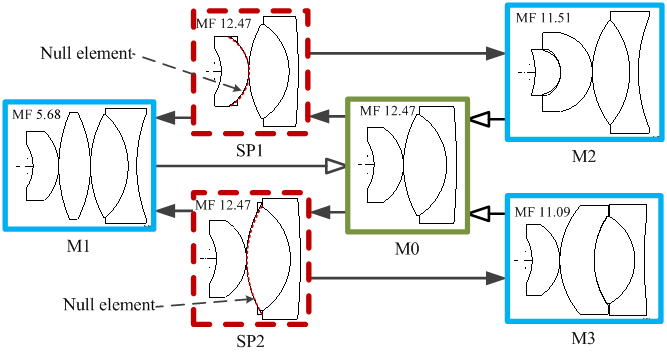
\includegraphics[scale=0.6]{chapter-3/figures/WideAngleSwitch.png}
    \caption{Switching between minima (blue boxes) using SPC. Extraction of the second element from M1, M2, or M3 results in the system M0 (hollow arrows). Starting from M0, two routes, each having an SP, lead to three different minima (solid arrows). The two SPs shown in dashed red boxes can be found both by the general and by the special version of SPC. In SP1, the null-element has the same curvature as the second surface of M0; in SP2, it has the same curvature as the third surface of M0 (because of two zero thicknesses, we see there three overlapping surfaces, marked by red dashed line).}
    \label{fig:wideangleSwitch}
\end{figure}

Optimization can be trapped in the sub-optimal minima M2 and M3, which are significantly worse than M1. However, the global minimum M1 can be rapidly obtained with SPC from both of them. In M2 or M3, the second element is extracted first and then the SPC method is applied (suitable candidate lenses for extraction are in general weaker-power lenses that seem to have little function). After extraction and optimization, both solutions became the M0 system shown in the green box in Figure \ref{fig:wideangleSwitch} Then two SP systems, SP1 and SP2 in Figure \ref{fig:wideangleSwitch} (in the red dashed boxes), were constructed from M0 by adding a null element in between the first and the second lens (i.e., at the position of extraction). From each SP system, two local minima can be found after optimization. In this case, both SP systems led on one side to the same minimum, the global minimum M1. On the other sides, the two SPs lead to M2 and M3. In fact, from any of these three minima, the other two can be found by a switching operation. In this example, different ways of using the SPC method described in Chapter 2 are demonstrated: firstly, the SPC method can systematically find new solutions with more lenses (M1, M2, and M3) from a simpler system (M0); secondly, extracting and then adding lenses with the SPC can lead to different minima in a systematic way. This possibility of switching between different local minima is a typical property of the SPC.
%%%%%%%%%%%%%%%%%%%%%%%%%%%%%%%%%%%%%%%%%%%%% Section %%%%%%%%%%%%%%%%%%%%%%%%%%%%%%%%%%%%%%%%%%%%%%%%
\section{Designing a pinhole system starting from a single lens} \label{chrom90d}

In the previous section it was seen how by using SPC different designs can be found systematically by increasing the number of lenses. By using this approach in combination with traditional methods it is possible to design an optical system starting with just one lens. This part shows how a pinhole lens similar to the one in Figure \ref{fig:widepinLens}(a) can be obtained from a single lens. The specifications are listed in Table \ref{table: sysspec}. The same merit function is used as before.

A global optimization was performed starting from a plane parallel plate. Only one singlet solution was obtained, with MF 576.30, as shown on the left in Figure \ref{fig:WideAngleDesign}(a). This singlet served as a basic element, providing optical power to the system \cite{LivshitsQA2013}. On this singlet SPC was performed by adding a zero-thickness glass element at the back surface. Two doublet minima were found, with MF 164.81 and MF 1783.94 (the latter one disappears if we replace EFL 3.5 mm by, e.g., EFL 3.0 mm). The better one (the first one) was chosen for the next design step. 

\begin{figure}[h!]
    \centering
    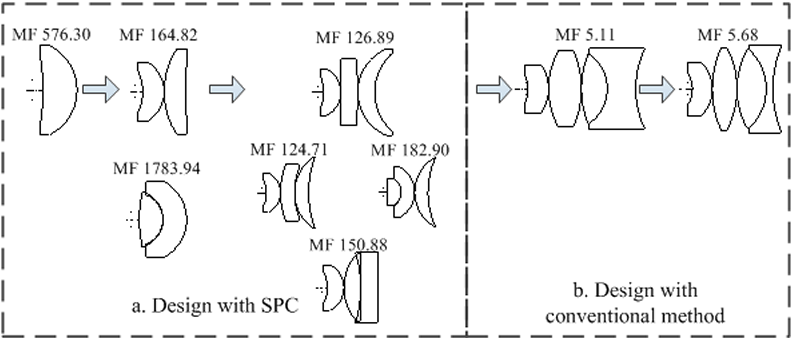
\includegraphics[width=1.0\textwidth]{chapter-3/figures/WideAngleDesign.png}
    \caption{Designing a wide-angle pinhole lens from one lens by combining SPC with conventional methods.}
    \label{fig:WideAngleDesign}
\end{figure}

With the same strategy, SPC was performed on four different surfaces of the doublet with MF 164.82 and four triplet minima were found (with merit function values 124.71, 126.89, 150.88, and 182.90, respectively). Only one type of glass was used for the steps mentioned above. In the next step, we continued with the best two minima using conventional design techniques: glasses were changed and the third lens was replaced by a cemented doublet to correct chromatic aberrations. The glasses were selected to be the same as the original system designed by Irina Livshits. When the glass were modified, the best minimum (MF 124.71) of the triplets encountered ray failure. However, the system with MF 126.89 still remained stable after changing the glass. Optimization with all curvatures and thicknesses as variables led to a system with MF 5.11 [Figure \ref{fig:WideAngleDesign}(b)]. By readjusting the thickness of the lenses for a more compact size, a system with the merit function value of 5.68 was obtained [see Figure \ref{fig:WideAngleDesign}(b)], which is identical to the original design in Figure \ref{fig:widepinLens}(a).

SPC is useful for dealing with minima created by monochromatic aberrations. It cannot deal directly with minima created by chromatic aberrations. However, since typically chromatic aberrations are less non-linear than monochromatic ones (e.g., unlike the Seidel aberrations, for axial chromatic aberration the thin-lens expressions are linear), the chromatic aberrations tend to create fewer new minima than the monochromatic
ones. As shown in this example, in the design process SPC can be easily combined with traditional approaches to handle chromatic correction.

In addition, four triplet minima were found with the SPC method in the search using only one glass, as shown in Figure \ref{fig:WideAngleDesign}(a). Both Global Synthesis \footnote{It is a proprietary global optimization algorithm of CODE V. The algorithm starts from the given system and explore solutions space for new configurations in a systematic manner.} and saddle point detection
(NETMIN \footnote{NETMIN is a tool developed in TU Delft to search for new local minima based on saddle point detection method. Detailed description can be found in Chapter \ref{method: spd}.}) have found only three minima (missing the one with the merit function value of 182.90). Therefore, in this example the SPC method has the advantage of being able to find more minima than the two methods used for comparison. 

%%%%%%%%%%%%%%%%%%%%%%%%%%%%%%%%%%%%%%%%%%%%% Section %%%%%%%%%%%%%%%%%%%%%%%%%%%%%%%%%%%%%%%%%%%%%%%%
\section{Decomposing a high-dimensional search for new minima in a succesion of one-dimensional searches}  \label{chrom60d}

It is mentioned in the previous section that the SPC found more system candidates compared to the Global Synthesis of CODE V and the saddle point detection algorithm. However, in the examples the number of minima found in the landscape is small. In this section it is investigated whether the performance of SPC is still good when more minima are present in the landscape.

In order to generate more minima, the FOV of the triplet system was reduced to 60° while the other specifications remained as that given in Table \ref{table: sysspec}. The reason why a reduced
field leads to more minima will be discussed in the next section.
As in Figure \ref{fig:WideAngleDesign}(a) only one type of glass was used, the variables were only the curvatures. The same default CODE V merit function was used, and, for the purpose of this study, the control of edge thickness was disabled. All lenses are in contact (i.e., all air spaces between lenses have zero thickness). The thicknesses of all lenses in a minimum system are set equal, in order to avoid the multiple appearance of essentially the same minima (with similar curvatures, but different lens thicknesses) that would unnecessarily complicate the study \cite{HouProc2015}.

For a better understanding of the results, in addition to the comparison of minima, it is also useful to compare the saddle points obtained using SPC with those obtained using the saddle point detection algorithm (realized by the program NETMIN). For SPC there are the options of inserting in the existing minimum either a glass null-element (i.e., inserting a lens) or an air null-element (i.e., splitting a lens). If the zero-thickness glass element was used, the saddle points resulting from the SPC scan would still have a zero-thickness lens, whereas the saddle points detected with NETMIN will have finite thicknesses for all lenses. This is because that the NETMIN starts from existing minima with non-zero thickness element and searches for the saddle points. The saddle points obtained from the two methods can not be directly compared due to the thickness differences of the lens element. In our study all lens elements are set to be in contact. In this case, the saddle points detected with NETMIN will have zero air spaces. It is therefore better for comparison to study the performance of the SPC when air null elements are used. Splitting lenses with SPC leads to saddle points with a zero distance between lenses, which are directly comparable with the saddle points from NETMIN. For performing SPC with a zero-thickness air element, the thickness of the lens, which will be split, is first doubled. Then the system is re-optimized to a minimum, and a zero-thickness air element is inserted in the middle of the lens. As mentioned in section \ref{section: SPC recommendation}, the example of Cooke triplet shows that the minima are different between applying zero-thickness glass and zero-thickness air space constructions. Therefore, both approaches are recommended to be used. However, in this example, it turned out that SPC with zero-thickness glass does not give more local minima than using zero-thickness airspace. For simplicity and better comparison, the SPC result using zero-thickness air space is shown. 
\begin{figure}[h!]
    \centering
    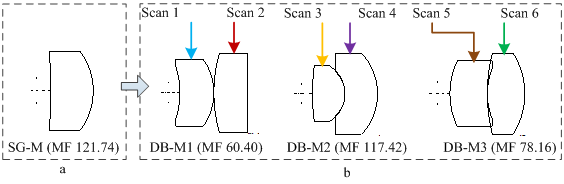
\includegraphics[width=0.8\textwidth]{chapter-3/figures/Single2Double.png}
    \caption{SPC by inserting a zero-thickness air element. (a) Singlet solution. (b) The three doublet minima that result from the singlet are the starting minima for the scans shown in Figure \ref{fig:tripletnetwork}.}
    \label{fig:single2double}
\end{figure}
As previously, we started with a single optimized lens [SG-M shown in Figure \ref{fig:single2double}(a)] and three doublets were obtained with the SPC [shown in Figure \ref{fig:single2double}(b)]. The three doublets DB-M1, DB-M2, and DB-M3 have a total of six lenses.  Each of the six lenses was used to generate an SPC scan that led to triplet minima. The colored arrows in Figure \ref{fig:single2double}(b) indicate the lenses that are split (after the thickness doubling that is not shown here) in the corresponding scan.

Figure \ref{fig:tripletnetwork} shows the minima and SP systems found in the triplet design space with NETMIN and Global Synthesis (Global Synthesis has found nine out of 10 minima, missing the minimum M6). Five curvatures were used as variables, and the curvature of the last surface was controlled by a \textit{Solve} in CODE V to keep the effective focal length constant.

A significant result of this search is that all 10 triplet minima shown in Figure \ref{fig:tripletnetwork} were also obtained with SPC starting from the three doublets in Figure \ref{fig:single2double}. Eleven SP systems were obtained from the six one-dimensional SPC scans. Different scans found different numbers of SPs. For instance, in Scan 2 there were four SPs (SP1, SP2, SP7, and SP8 in Figure \ref{fig:tripletnetwork}), whereas in other scans, only one or two SPs were found. The 10 minima resulted from the 11 SP systems by optimization on both sides of the saddle. Saddle-point systems and minima obtained from the same scan are connected in Figure \ref{fig:tripletnetwork} with lines having the same color. In the figure, when gradually increase the FOV, M1 corresponds to the system leading to the final design in the 110° case [MF 126.89 in Figure \ref{fig:WideAngleDesign}(a)]. However, in this case its MF value of 61.14 is not the smallest one in Figure \ref{fig:tripletnetwork}.

NETMIN has found the extra SP system SP12, which cannot be found by SPC. This SP system connects with a dashed link the minima M3 and M9 in Figure \ref{fig:tripletnetwork}. However, there is sufficient redundancy in the SPC approach, and both M3 and M9 also result from other SP systems which are found by SPC. Therefore the lack of ability of SPC to find SP12 is not critical.

Since there are five variables, with general global optimization tools this search has to be performed in a five-dimensional space. In this example, however, all minima found with other methods were also found with SPC, where the five-dimensional search was replaced by six one-dimensional searches. Replacing a high-dimensional search for new minima by a succession of one-dimensional searches reduces the complexity of the search significantly.

The example discussed above shows the utility of the feature of the optical merit function landscape that enables the decomposition of the search for many of the minima in simpler steps. The feature means that minima and saddle points are all connected, and the saddle points can be constructed by SPC. This example has the advantage that in this case the feature mentioned above can be observed in a pure form, without interference from other features (e.g. the minima are not connected by saddle points that can be constructed) of the landscape. However, in general other features, which deserve further study for a better understanding, may also play a role. Therefore, it cannot be expected that we can always find all minima using SPC. Nevertheless, even when other features are present, examples studied so far show that SPC can lead to satisfactory results.

For instance, when the search described in Figure \ref{fig:tripletnetwork} was repeated with modified wavelength specifications, SPC found 11 minima and Global Synthesis found 10 (see Figure \ref{fig:TripletMonoNetwork}). Among these minima, eight, including the best five were found by both methods. For the four minima that were missed by SPC, two of them are unphysical (minima 12 and 14, they have either negative or zero back focal length that cannot be corrected, but should be prevented with an additional constraint). These unphysical solutions also have a merit function more than 4 times and more than 50 times that of the best solution. The other two minima missed by SPC (minima 13 and 15) have a merit function 40 times and 8 times that of the best solution. NETMIN found all four solutions missed by SPC, and Global Synthesis found two of them.

% \begin{figure}[h!]
%   \begin{adjustbox}{addcode={%
%     \begin{minipage}{\width}}{%
%     \captionsetup{margin=0em}
%     \caption{Network of minima (solid boxes) and SP systems (dashed boxes) in the 60° landscape, where the other specifications are the same as in Table \ref{table: sysspec}. Eleven SP systems result from six SPC scans (each color represents one scan). Optimization starting at these SP systems leads to all 10 minima that were obtained with NETMIN and Global Synthesis. If in any of these 11 SPs we remove the null-element of the corresponding scan (this does not affect the ray paths or the MF), we obtain the starting doublet of the scan. The null elements are marked by crosses with the corresponding color. This figure shows why the lens design landscape is different from general global optimization landscapes: because of the close relationship that exists between local minima of a design problem (here the 10 triplet minima) and local minima with one lens less (here the starting doublets).}\label{fig:tripletnetwork}
%     \end{minipage}},rotate=90,center}
%     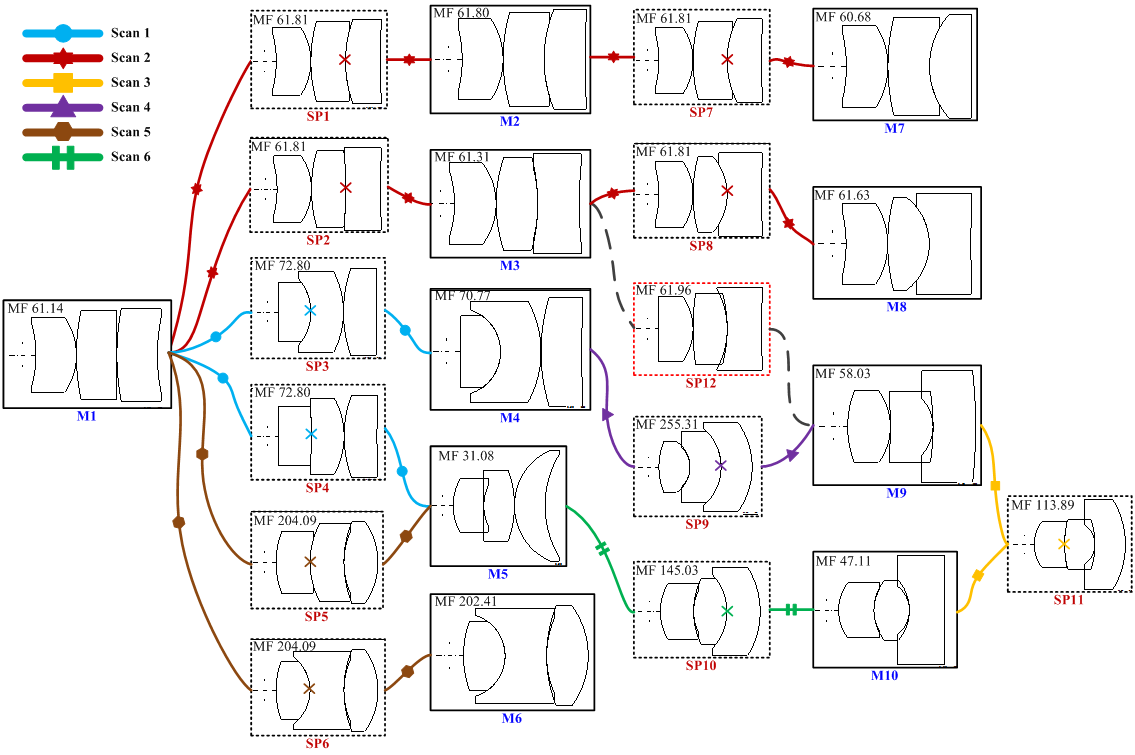
\includegraphics[scale=0.5]{chapter-3/figures/TripletNetwork.png}
%   \end{adjustbox}
% \end{figure}

\begin{figure}[h!]
    \centering
    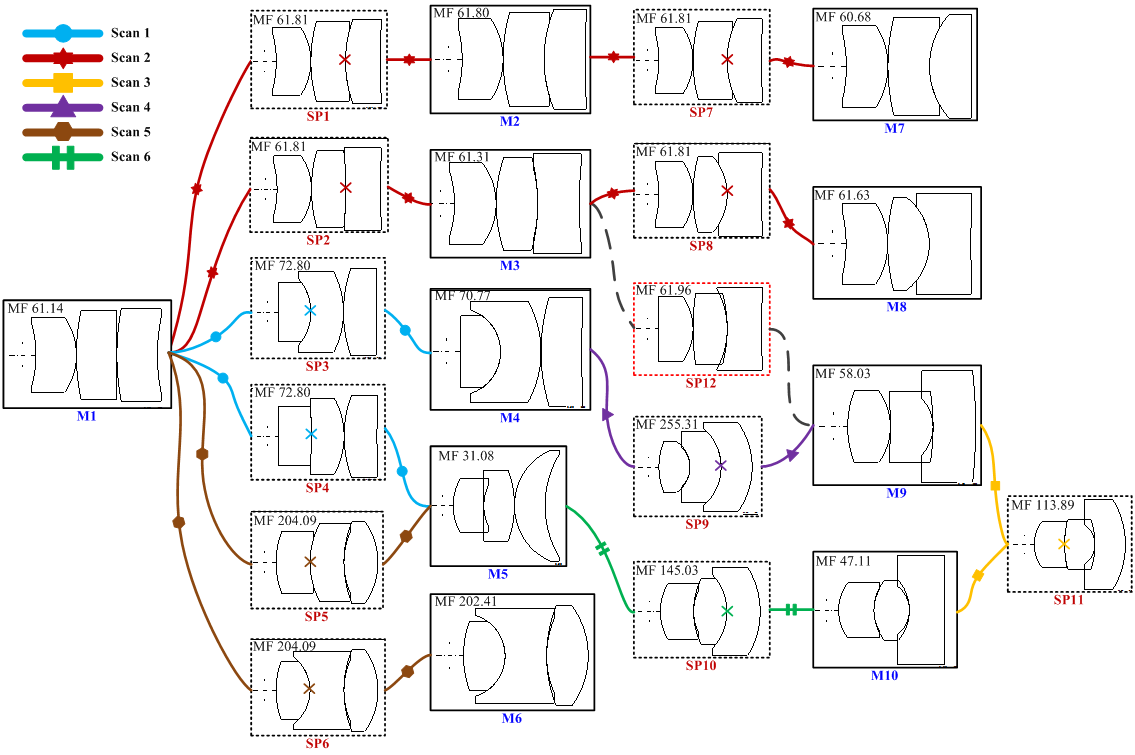
\includegraphics[scale=0.41]{chapter-3/figures/TripletNetwork.png}
    \caption{Network of minima (solid boxes) and SP systems (dashed boxes) in the 60° landscape, where the other specifications are the same as in Table \ref{table: sysspec}. Eleven SP systems result from six SPC scans (each color represents one scan). Optimization starting at these SP systems leads to all 10 minima that were obtained with NETMIN and Global Synthesis. If in any of these 11 SPs we remove the null-element of the corresponding scan (this does not affect the ray paths or the MF), we obtain the starting doublet of the scan. The null elements are marked by crosses with the corresponding color. This figure shows why the lens design landscape is different from general global optimization landscapes: because of the close relationship that exists between local minima of a design problem (here the 10 triplet minima) and local minima with one lens less (here the starting doublets).}\label{fig:tripletnetwork}
\end{figure}

Despite the fact that SPC cannot find four (poor-quality) minima directly, it turns out that by using the switching strategy described earlier it is easy to escape from any of them if optimization is trapped. Eliminating a lens from any of these poor-quality minima leads to one of the three doublets. From these doublets, better minima can be obtained with SPC.
\begin{figure}[h!]
    \centering
    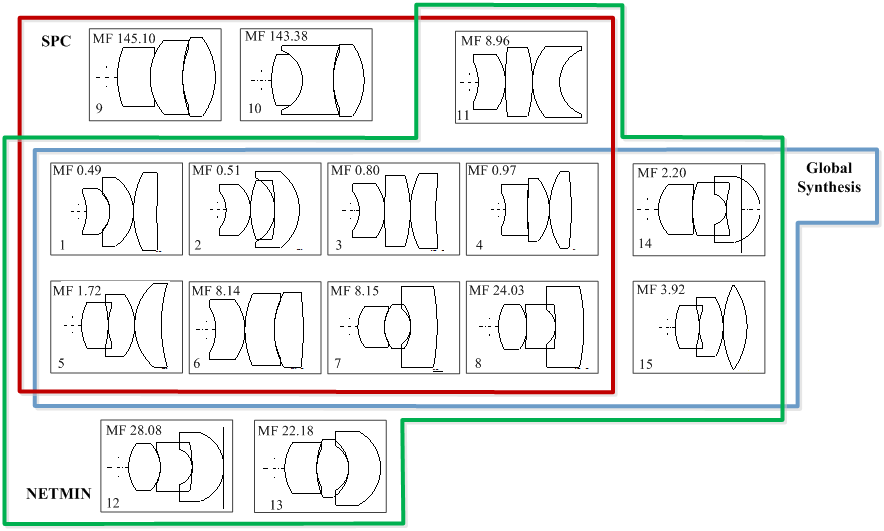
\includegraphics[width=1.0\textwidth]{chapter-3/figures/TripletMoNoNetwork.png}
    \caption{Minima found with SPC (red box), Global Synthesis (blue box), and NETMIN (green box) in a monochromatic run. Minima 12 with MF 28.08 and Minima 14 with MF 2.20, whose image planes are inside or coincide with the last lens, are unphysical. The five minima with the lowest MF value (numbered from 1 to 5) are found by all three methods. Edge thickness violations have been disabled in this search.}
    \label{fig:TripletMonoNetwork}
\end{figure}

However, for understanding the potential and the limitations of SPC it is useful to examine why SPC was not able to reach these four minima. SPC is based on the assumption that small changes in lens thicknesses do not affect good designs significantly, i.e., that good minima continue to exist as minima when a reasonably small non-zero thickness is replaced by zero. This assumption is similar to the one at the basis of the well-known thin-lens aberration theory. In earlier days of lens design, primary aberration formulas using zero thickness were used to predict qualitatively the existence of good designs.

It turns out that the minima that were not found by SPC only exist for certain non-zero thickness values and do not have a zero-thickness equivalent. However, the existence of these minima does not contradict our assumption that using SPC can obtain satisfactory solutions, because these were not among the best solutions. In the numerical experiment, final solutions have the same thickness for each lens element (1.5 mm). Since in the SPC procedure the practical design is always obtained after increasing the zero-thickness of a null element, it is not possible to reach minima that for which there are no local minima where the corresponding lens to the null element has zero thickness. In NETMIN and Global Synthesis searches the lens thicknesses were kept constant. This typical behavior is illustrated in Figure \ref{fig:thicknesschange}(a) and (b). In the system in Figures \ref{fig:thicknesschange}(a) found by SPC, the thickness of the first lens is 1.5 mm. By starting with a zero-thickness null-element as the first lens as in Figure \ref{fig:thicknesschange}(b), increasing the thickness leads to the system in Figure \ref{fig:thicknesschange}(a). By decreasing the thickness of the first lens of the system in Figure \ref{fig:thicknesschange}(a), the system in Figure \ref{fig:thicknesschange}(b) is obtained. In contrast, in the system in Figure \ref{fig:thicknesschange}(c) found by NETMIN but not by SPC, when the thickness of the first lens is decreased ray failure occurs and a system with zero-thickness element cannot be obtained. However, systems like the one in Figure \ref{fig:thicknesschange}(c) have low stability. A small perturbation on the system in Figure \ref{fig:thicknesschange}(c) will lead to the system in Figure \ref{fig:thicknesschange}(a).

\begin{figure}[h!]
    \centering
    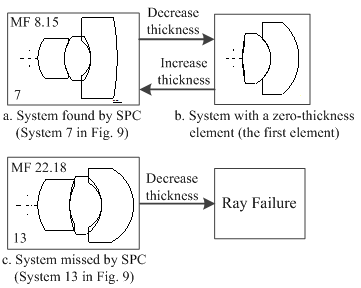
\includegraphics[scale=0.7]{chapter-3/figures/thicknesschange.png}
    \caption{Increasing the thickness of the first element of system (b) results in system (a), and vice versa. System (b), which is obtained by the SPC, is a minimum with a zero-thickness element. System (c), which is missed by the SPC, does not have a corresponding zero-thickness pair. A small perturbation on system (c) will lead to system (a).}
    \label{fig:thicknesschange}
\end{figure}


%%%%%%%%%%%%%%%%%%%%%%%%%%% Section %%%%%%%%%%%%%%%%%%%%%%%%%%%%%%%%%%%%%%%%%%%
\section{Effect of changing the field of view on the landscape}
In Section \ref{chrom90d} and \ref{chrom60d} it was found that when the field of view is reduced, more minima can be found in the design space. This happens for two reasons. First, when design specifications (e.g., FOV or entrance pupil diameter) are modified, the distances in the design space between minima and SPs change
and therefore the merit function landscape also changes. As can be observed in numerical experiments, when a minimum and an SP with Morse Index $1$ collide, they both disappear. Alternatively, such a pair can appear when specifications are changed. Similarly, two minima with an SP between them can be replaced by one minimum, and two SPs with a minimum between them can be replaced by an SP. This can be explained mathematically by the conservation of the topological degree of the MF landscape \cite{vanTurnhoutThesis2009} \cite{KoornwinderTopologicaldegree}. The topological degree of a critcal point is the sign of the determinant of the Hessian matrix in that point. The degree of a critical point is thus $(-1)^{Morse Index}$. A minimum has a topological degree of $+1$ and an SP with Morse Index $1$ has a topological degree of $-1$. The sum of the topological degrees remain constant under perturbation such as changing the FOV. Second, when the FOV is increased ray failure appears more easily, and the region of ray failure expands in the design space. Because certain minima and SPs which exist for lower FOV cross the border of the ray failure region and disappear, fewer of them are found at large FOV.

 When varying the FOV of the systems in shown Figure \ref{fig:tripletnetwork}, it is observed the number of solutions with the FOV as shown in Figure \ref{fig:FOVvarying}. Three different FOVs are chosen: 110°, 90° and 60°. Six solutions were obtained for 110°, five for 90° and ten for 60°. From Figure \ref{fig:FOVvarying}, it is seen that some system shapes exist in all the three FOV configurations. However, other system shapes only exist in the specific FOV range.
For FOV 60°, five new systems, which did not exist for larger field (second row for the 60° systems in Figure \ref{fig:FOVvarying}). The dashed boxes in Figure \ref{fig:FOVvarying} mark the missing systems which exist in other FOV specifications. As mentioned in the previous paragraph, the appearance and disappearance of the systems can be explained by the change of the merit function landscape. 

\begin{figure}[h!]
    \centering
    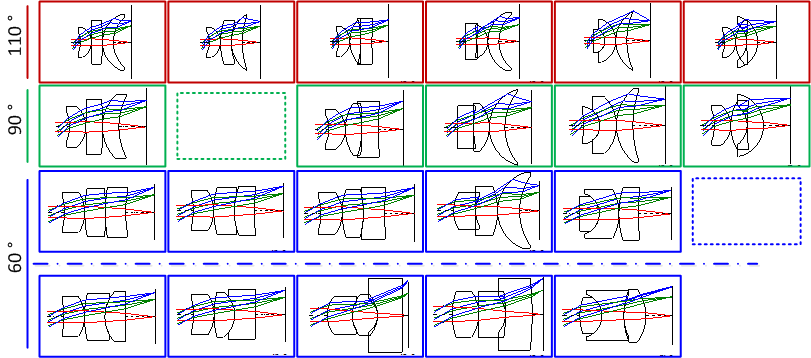
\includegraphics[width=1.0\textwidth]{chapter-3/figures/FOVvarying.png}
    \caption{For different field of view, the number of solutions is different. Systems with 110° FOV have six solutions marked by the red colour; Systems with 90° have five solutions marked by the green colour; Systems with 60° marked by the blue colour. The dashed boxes mark the missing systems.}
    \label{fig:FOVvarying}
\end{figure}

These phenomena can also be observed by examining the SPC scan curves. Figure \ref{fig:phasechange_field} refers to Scan 2 of Figure \ref{fig:tripletnetwork} where five minima are linked by four saddle points, and the FOV is 60°. In Figure \ref{fig:phasechange_field}, the scans were performed in different FOV settings: the FOV of the system increases from 50° [Figure \ref{fig:phasechange_field}(a)] to 90° [Figure \ref{fig:phasechange_field}(d)]. With the increase of the FOV, the ray failure region (shown as shaded area) is seen to expand. Two SPs are found at 70° [Figure \ref{fig:phasechange_field}(c)], however, at 90° [Figure \ref{fig:phasechange_field}(d)] the most left SP disappears into the ray failure region.
\begin{figure}[h!]
    \centering
    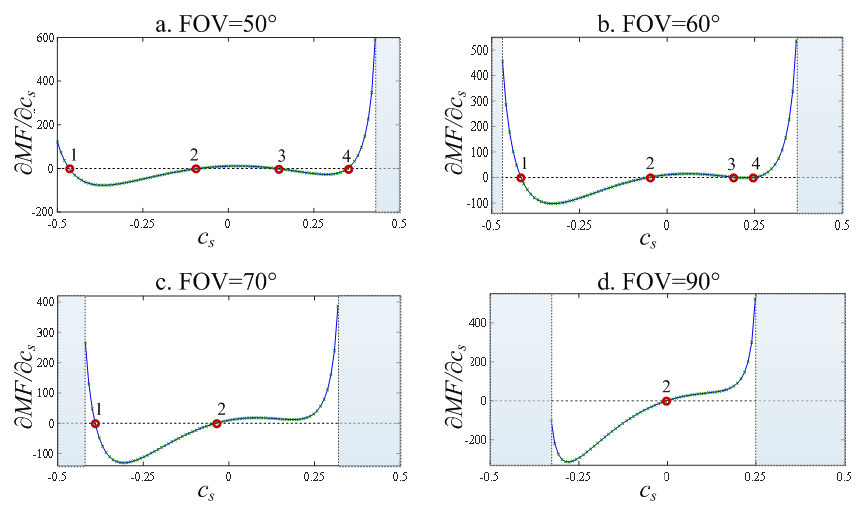
\includegraphics[width=.85\textwidth]{chapter-3/figures/PhaseTransition_field.png}
    \caption{SPC scan curves for different values of the FOV. Shaded areas are ray failure regions. The scan curves are obtained in the same way as the one shown in Figure \ref{fig:SPCscan}. Saddle-point curvatures are marked by red circles. With the increase of the FOV, SP 1 disappears in the ray failure region. SPs 3 and 4 merge with the minimum between them, and are replaced by a saddle point (not shown) that is not constructible with SPC.}
    \label{fig:phasechange_field}
\end{figure}

A different kind of change is also observed. At 50° [Figure \ref{fig:phasechange_field}(a)] four SPs can be found. However, at larger fields the third and fourth SP first move closer [Figure \ref{fig:phasechange_field}(b)], merge and then disappear [Figure \ref{fig:phasechange_field}(c) and (d)]. 

By optimizing from the SPs, at 50° it is found that the last two SPs lead on one side of the saddle to the same minimum. While changing the FOV in small steps, it is possible to keep track of the two SPs and one minimum by keeping the norm of the gradient to zero via minimization. The process is elaborated in Figure \ref{fig:systemdie}. When the FOV increases from 50° to 60°, it is seen that the Euclidean distances between the SPs and minimum reduce. Hence the critical points are getting closer in the high-dimensional design space. At 70°, it is no longer possible to find SPs via an SPC scan. However, it is still possible to obtain the merged point by keeping the norm of the gradient to zero at the vicinity of the previous critical points. From Figure \ref{fig:systemdie}, it is seen that the original two SPs and one minimum merge into one SP with a merit function value of 74.92. It is an SP without any null element, hence it cannot be constructed using SPC. This shows how two SPs and one minimum merge into one SP while the FOV increases. 

\begin{figure}[h!]
    \centering
    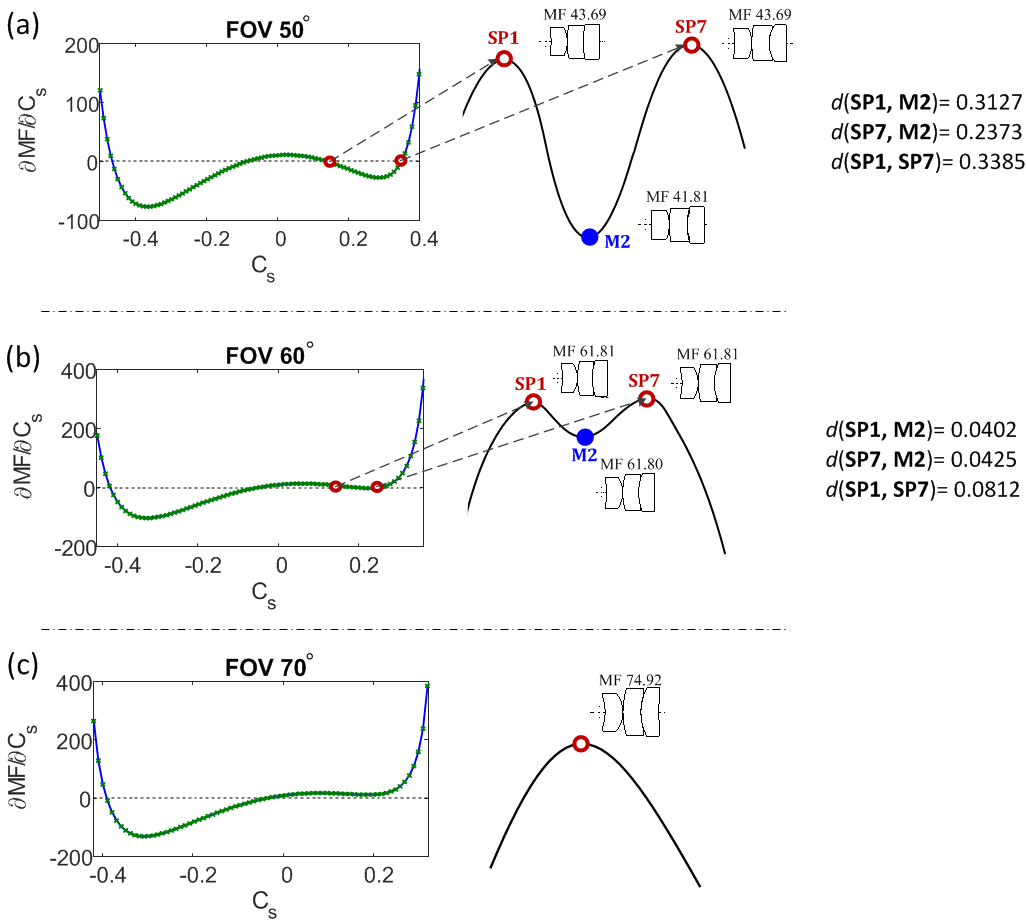
\includegraphics[width=0.8\textwidth]{chapter-3/figures/SystemDie.png}
    \caption{Merging of two SPs and one minimum when the FOV increases, from Figure (a) to Figure (c). In the SPC scan curves, the two saddle points get closer and then disappear. The two SPs and one minimum in between merge into one SP. The decreasing Euclidean distances also indicates the merging.}
    \label{fig:systemdie}
\end{figure}

The process may also happen in a reverse way when FOV increases. In Figure \ref{fig:systemborn}, the two SPs on the left side of the scan curve are investigated: at 54°, SP8 and SP2 both lead to M9 when optimizing on one side. However, when the FOV increases to 56°, the two SPs are connected to M3 instead of M9. The minimum M9 is connected to M3 via SP12. M3 and SP12 cannot be obtained when the FOV is 54°. It indicates that when FOV increases, M9 splits into two local minima (M3 and M9) and an SP (SP12). When the FOV increases to 60°, the Euclidean distance between M3 and SP12 also increases from 0.1148 to 0.2611. 

Besides merging or splitting, it is also found that in some special situations, when FOV increases, both approaching and distancing\footnote{When mentioned merging, we observed that a pair of points approach each other and reach a situation where they cannot be distinguished anymore. When mentioned splitting, we observe that one point split into two and they move away from each other. When this happens in a continuous way with a change of the system setting (e.g. FOV), approaching and distancing is used to describe the behaviour of the two points.} happens for the same pairs. Figure \ref{fig:systemreborn} illustrates a scenario when a glass null element was used as an SPC scan element. The FOV is increased from 60° to 110°, where three steps (60°, 90° and 110°) are plotted in the figure. At 60°, two saddle points were found by the scan. Both of them lead to a common minimum at one side (illustrated on the right of the scan curve). With the increasing of the FOV, the two saddle points become closer in the design landscape: the Euclidean distance reduces from 0.0785 to 0.0023 when the FOV increases from 60° to 90°. At this phase, a much smaller step size of the scan is necessary to be able to find the saddle point. After the FOV increased to 110°, the Euclidean distance between the two increases from 0.0023 to 0.0217. As a result, the tendency of the merging of the two saddle points changes to splitting. 

It has been seen in the aforementioned three examples that the change of the design landscape can be dynamic and unpredictable. When a certain design specification changes, it essentially alters the design landscape. This change may affect the number of saddle points and minima, which can be obtained with the SPC approach. Nevertheless, for the given examples, redundancy of the saddle point - minimum links also reduces the risk of missing solutions with the SPC approach. All the good solutions were obtained with the SPC method.

\begin{figure}[h!]
    \centering
    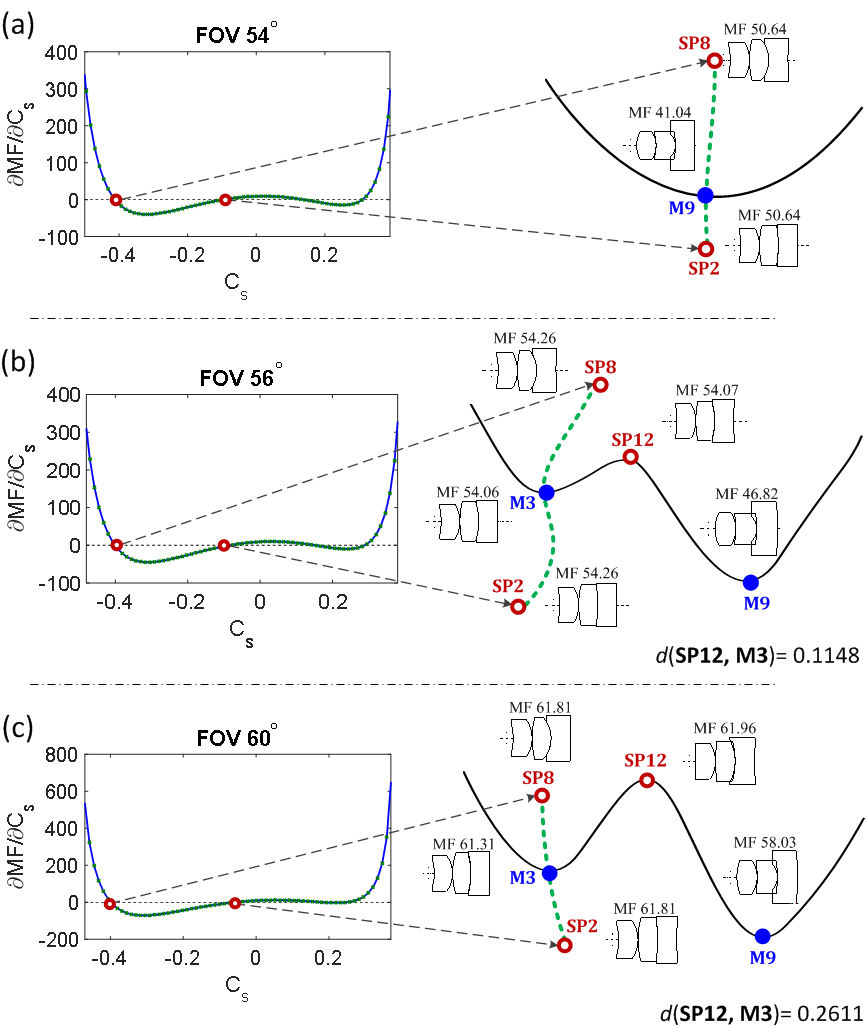
\includegraphics[width=0.75\textwidth]{chapter-3/figures/SystemBorn.png}
    \caption{A minimum spliting into SPs and minimum when FOV increases. From (a) to (c), the FOV increases. M9 splits into two SPs and one minimum. The connection between SPs and minima are altered: at 54°, SP8 and SP12 connect to M9; at 56°, SP8 and SP12 connect to M3.}
    \label{fig:systemborn}
\end{figure}

\begin{figure}[h!]
    \centering
    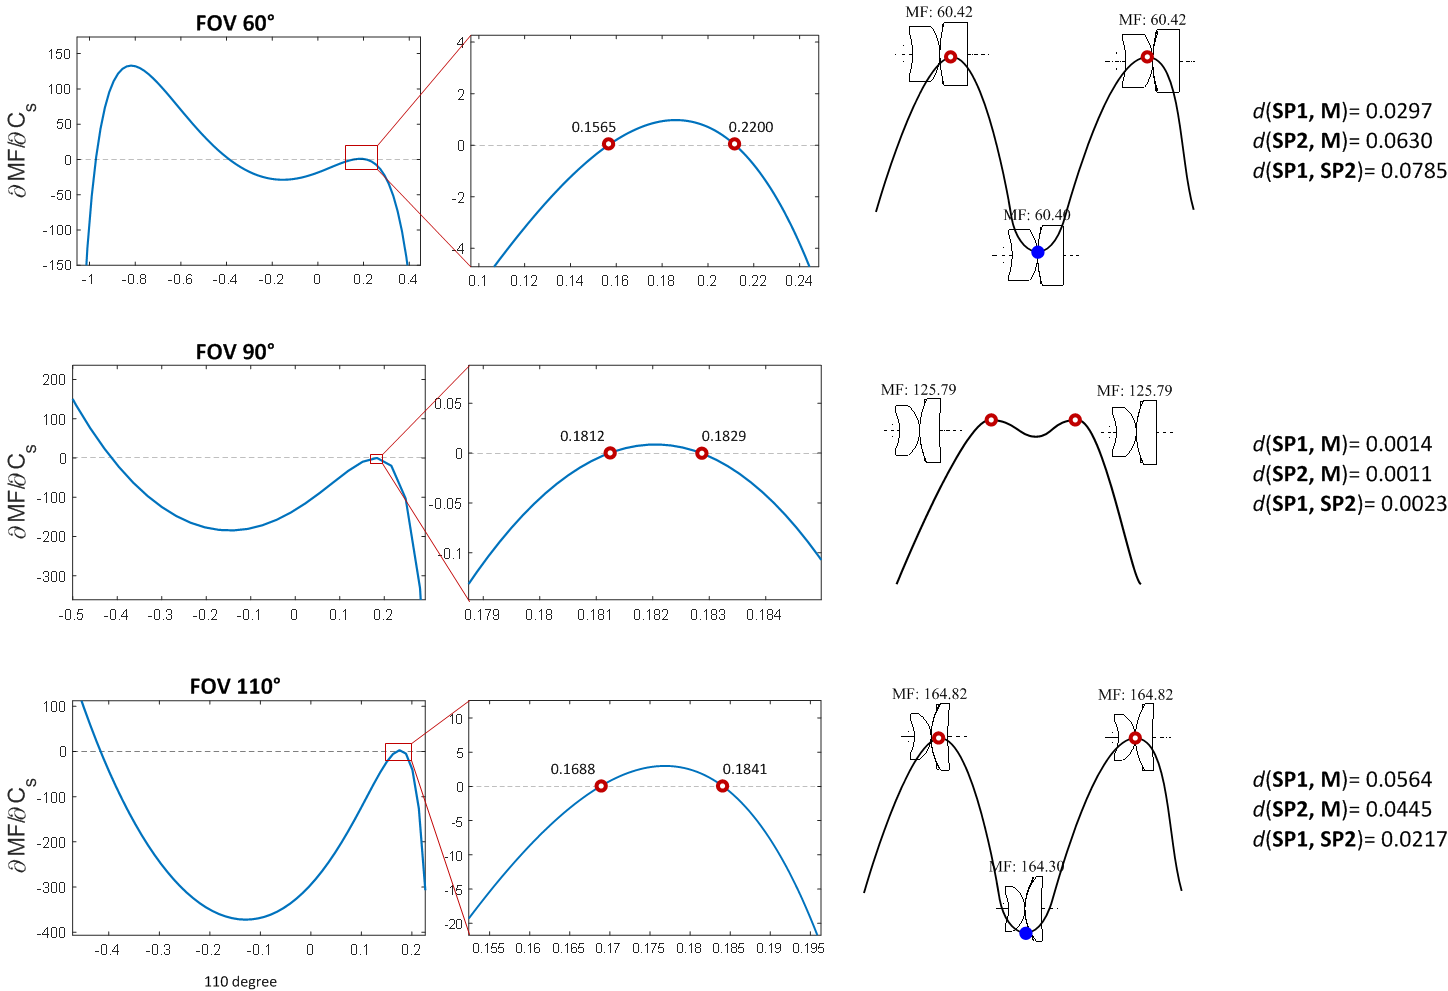
\includegraphics[width=0.8\textwidth]{chapter-3/figures/SystemReborn_vt.png}
    \caption{A glass null-element SPC scan is performed on DB-M1 from Figure \ref{fig:single2double}. The scan position is between the two lens elements. When the FOV increases from 60° to 110°, the two saddle points on the right first get closer, and then further apart. This phenomenon can be observed from the SPC scan curve as well as from the Euclidean distances between the two.}
    \label{fig:systemreborn}
\end{figure}
%%%%%%%%%%%%%%%%%%% Section %%%%%%%%%%%%%%%%%%%%%%%%%%%%%

\section{Discussion and conclusion}
The design landscape of a wide-angle pinhole lens and its closely related optimization landscape are investigated in this chapter. Several observations that result from this study have a more general validity. Switching between minima with SPC introduced in Subsection \ref{cp2-switching}, is applied to the pinhole lens as shown in Figure \ref{fig:wideangleSwitch}. It can be used in other design tasks as well to avoid the trapping of the optimization in a sub-optimal solution. Combining SPC with conventional design methods, as shown in Figure \ref{fig:WideAngleDesign}, can lead to good complex designs starting from simpler ones \cite{LivshitsSP2014}.

The lens design landscape is different from general global optimization problems because of the close relationship that often exists between the local minima of a design problem and local minima with one lens less. Figure \ref{fig:tripletnetwork} is particularly useful to illustrate this structure due to the special choices that were made in the corresponding search (lenses in contact, use of air null elements). The systems SP1–SP11 are triplet saddle points, but if the air null-element of the corresponding scan (a pair of surfaces that has no influence at all on the rays or on the merit function) is removed, they become doublet minima. However, when these doublet minima with an extra null-element are optimized on both sides of the resulting saddle, they lead to the triplet minima M1–M10. In the search shown in Figure \ref{fig:tripletnetwork}, these 10 triplet minima are all minima found in the landscape with other methods such as NETMIN and CODE V that were used for comparison. A scenario where this structure holds for all minima has been previously encountered \cite{PascalTriplet2009}. The corresponding landscape is dominated by spherical aberration. The wide angle examples discussed here show that the scenario, where this structure is present for most of the minima, can be much more general.

% HZ: the structure is a structure that all minima are connected via saddle points, and these saddle points can be constructed using SPC. Having a trans-dimensional structure of the minima and saddle point does not ensure the connection of the saddle point and minima within the same dimension. Local or global structure?

The example shown in Figure \ref{fig:tripletnetwork} has the advantage that the special structure can be observed in a pure form, where all minima and saddle points are connected and the saddle points can be constructed using SPC. Interference of other features can also be present as seen in the examples: Figure \ref{fig:thicknesschange} indicates that some minima does not have a corresponding system with a zero-thickness element, therefore cannot be obtained following the SPC procedure; Figure \ref{fig:phasechange_field} shows that saddle point which cannot be constructed with SPC are present. In these examples, using SPC cannot always find all minima. Nevertheless, Figure \ref{fig:TripletMonoNetwork} shows an example where even in the presence of the aforementioned features of the landscape the five solutions with the lowest MF value found with other methods can still be found with SPC.

The example shown in Figure \ref{fig:phasechange_field} is a useful for understanding the transition in the local landscape where saddle points that can be constructed using SPC become ones that cannot be constructed using SPC. In an extreme case where none of the saddle points can be constructed using SPC, the landscape becomes a standard global optimization landscape which does not have the special structure we mentioned. The replacement of the SPs 3 and 4 in Figure \ref{fig:phasechange_field} by a saddle point, which cannot be constructed with SPC, shows that the landscape is locally transformed into such a standard global optimization landscape. The process is elaborated in Figure \ref{fig:systemdie}. However, the transition can also happen in the opposite direction if the process (in this case, descreasing the FOV) is reversed: a usual saddle point splits into two saddle points and a minimum in between, and in this case, the two saddle points can be constructed using SPC. This complexity of the design landscape dynamic is further explored in Figure \ref{fig:systemborn} and Figure \ref{fig:systemreborn}: When the FOV is increasing, a minimum splits into two minima and one saddle point; Two saddle points and a minimum first tend to merge and then tend to separate again. 

Based on the examples shown in this chapter, the complex dynamic of the design landscape can already be observed. However, the structure that enables SPC to obtain good solutions is stable. For systems that are more complex than those presented in this chapter the utility of SPC will be determined by its practical success, rather than by a detailed study of the entire landscape, which becomes difficult. Systems with bigger complexities are investigated in the next chapter. 

The replacement of high-dimensional searches by several one-dimensional searches plus local optimization can lead to a reduction of the complexity of the search. It can be essential for practical purposes. Compared to global optimization methods where multiple starting points are firstly chosen heuristically and then local optimization is applied, SPC operates in a more systematic way that starting points are provided based on constructed saddle points. In computer programs where the search for new solutions is automated, the general version of SPC could be combined with other methods. In the case of the special version of SPC this has already been achieved in the commercial software SYNOPSYS \cite{DilworthSP2012}. Excepting simple problems, no known global optimization method can guarantee finding all (good) solutions in a reasonable time, and SPC is no exception. However, high-quality designs have already been obtained with the special \cite{MarinescuSP2008}\cite{BociortPatent2010} and with the general versions \cite{LivshitsSP2014} of SPC. SPC will finally be validated if many high-quality designs will be obtained with this method.

%We have seen that in lens design we can find good solutions with SPC. This method could also be applicable in other design problems where the conditions described in Sections 3 and 4 of \cite{MVTurnhoutSPC15} or in the Appendix of \cite{BociortToyModel2010} are satisfied. In a different multi-parameter optimization problem, if there is a way to construct a
%saddle point in the design landscape, then in principle, it should be possible to follow the same procedure as in lens design to search for new solutions.


\references{dissertation}

